\chapter{(Example) Small-Gain theorem}\label{ch: SMT_example}
Consider an unknown plant $P$. Let $P_n$ be a nominal description of the plant and $W_u$ a description of its uncertainty. Assume for example that a \textit{multiplicative uncertainty model set} is used, so that $P$ belongs to the following set:
\begin{equation}
    M_m=\{
        P=P_n(1+W_u(z)\Delta(z)), \ \Vert \Delta \Vert_\infty < 1
    \}
\end{equation}
When you put together the controller $K$ and the plant $P$ with its (unstructured) uncertain description, you obtain a block diagram like the following: 

\begin{figure}[h]
    \centering
    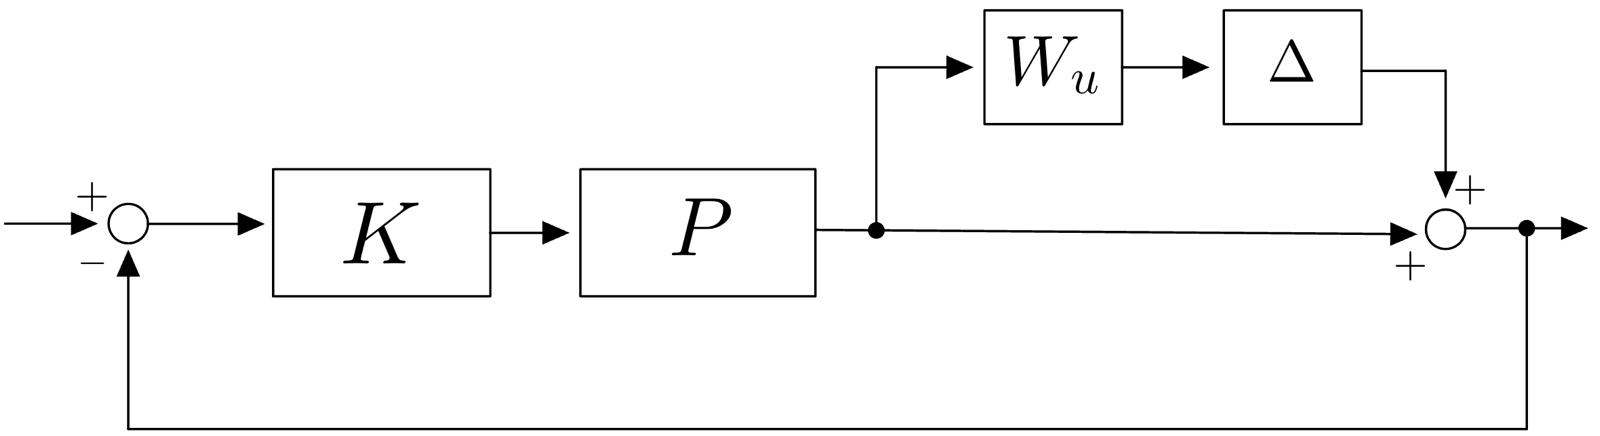
\includegraphics[scale=0.23]{img/uncertainFCS.jpg}
    \caption{Uncertain FCS structure}
    \label{fig:uncertainFCS}
\end{figure}

\noindent
If we use the \textit{small-gain theorem}, we can assume that
\begin{align}
    &S_1=\Delta\\
    &S_2=\frac{-KP_nW_u}{1+KP_n}= {W_u}{T_n}
\end{align}
where $\Delta$ is stable by assumption, $W_u$ is also stable by assumption while $T_n$ is stable if $K$ stabilizes $P_n$ (nominal stability fulfilled). Then, $S_1$ and $S_2$ are stable by assumption. A condition on robust stability can be found, if the small gain theorem is applied: 

\begin{align}
    &\Vert {S_1}{S_2} \Vert_\infty = 
    \bigg\Vert 
        \Delta \frac{-KP_nW_u}{1+KP_n}
    \bigg\Vert_\infty \le \quad \textsf{(sub-multiplicativity)}\\
    &\le \Vert \Delta \Vert_\infty \cdot \bigg\Vert 
    \frac{-KP_nW_u}{1+KP_n}  
\bigg\Vert_\infty \le \bigg\Vert 
\frac{-KP_nW_u}{1+KP_n}  
\bigg\Vert_\infty < 1 \iff\\
&\iff \Vert W_u T_n \Vert_\infty < 1
\end{align}
\noindent
Then robust stability (stability for all the plants in $M_m$) is guaranteed if and only if
\begin{equation}
    \Vert W_u T_n \Vert_\infty < 1
\end{equation}